%%% LaTeX Template: Article/Thesis/etc. with colored headings and special fonts
%%%
%%% Source: http://www.howtotex.com/
%%% Feel free to distribute this template, but please keep to referal to http://www.howtotex.com/ here.
%%% February 2011
%%%
%%% Modified January 2016 by CDM

%%%  Preamble
\documentclass[11pt,letterpaper]{article}
\usepackage[margin=1.0in]{geometry}
\usepackage[T1]{fontenc}
\usepackage[bitstream-charter]{mathdesign}
\usepackage[latin1]{inputenc}					
\usepackage{amsmath}						
\usepackage{xcolor}
\usepackage{cite}
\usepackage{hyphenat}
\usepackage{graphicx}
\usepackage{float}
\usepackage{subfigure}
\usepackage{sectsty}
\usepackage[compact]{titlesec} 
\usepackage[tablegrid]{vhistory}
\usepackage{pbox}
\allsectionsfont{\color{accentcolor}\scshape\selectfont}

%%% Definitions
\definecolor{accentcolor}{rgb}{0.0,0.0,0.5} 
\newcommand{\teamname}{Team CheckUR5}
\newcommand{\productname}{Checkers-Playing UR5 Co-bot}
\newcommand{\coursename}{CSE 4317: Senior Design II}
\newcommand{\semester}{Spring 2023}
\newcommand{\docname}{Detailed Design Specification}
\newcommand{\department}{Department of Computer Science \& Engineering}
\newcommand{\university}{The University of Texas at Arlington}
\newcommand{\authors}{Nimita Uprety \\ Patricia Rojas \\ Hoang Ho \\ Kevin Vu \\ Joanna Huynh}

%%% Headers and footers
\usepackage{fancyhdr}
	\pagestyle{fancy}						% Enabling the custom headers/footers
\usepackage{lastpage}	
	% Header (empty)
	\lhead{}
	\chead{}
	\rhead{}
	% Footer
	\lfoot{\footnotesize \teamname \ - \semester}
	\cfoot{}
	\rfoot{\footnotesize page \thepage\ of \pageref{LastPage}}	% "Page 1 of 2"
	\renewcommand{\headrulewidth}{0.0pt}
	\renewcommand{\footrulewidth}{0.4pt}

%%% Change the abstract environment
\usepackage[runin]{abstract}			% runin option for a run-in title
%\setlength\absleftindent{30pt}			% left margin
%\setlength\absrightindent{30pt}		% right margin
\abslabeldelim{\quad}	
\setlength{\abstitleskip}{-10pt}
\renewcommand{\abstractname}{}
\renewcommand{\abstracttextfont}{\color{accentcolor} \small \slshape}	% slanted text

%%% Start of the document
\begin{document}

%%% Cover sheet
{\centering \huge \color{accentcolor} \sc \textbf{\department \\ \university} \par}
\vspace{0.5 in}
{\centering \huge \color{accentcolor} \sc \textbf{\docname \\ \coursename \\ \semester} \par}
\vspace{0.25 in}
\begin{figure}[h!]
	\centering
   	
\includegraphics[width=0.60\textwidth]{images/Transparent_CheckUR5.png}
\end{figure}
\vspace{0.25 in}
{\centering \huge \color{accentcolor} \sc \textbf{\teamname \\ \productname} \par}
\vspace{0.25 in}
{\centering \large \sc \textbf{\authors} \par}
\newpage


%\vspace{1 in}
%\centerline{January 13th, 2012}
%\newpage

%%% Revision History
\begin{versionhistory}
  	\vhEntry{0.1}{2.01.2023}{HH}{document creation}
  	\vhEntry{0.2}{2.24.2023}{HH|KV|JH|PR|NU}{complete draft}
  	\vhEntry{0.3}{2.24.2023}{HH|KV|JH|PR|NU}{release candidate 1}
        \vhEntry{0.4}{5.10.2023}{HH|KV|JH|PR|NU}{final draft}
\end{versionhistory}
\newpage

%%% Table of contents
\setcounter{tocdepth}{2}
\tableofcontents
\newpage

%%% List of figures and tables (optional)
\listoffigures
\listoftables
\newpage

%%% Document sections
\section{Introduction}
% Your introduction should describe your product concept in sufficient detail that the architectural design will be easy to follow. The introduction may include information used in the first sections of your SRS for this purpose. At a minimum, ensure that the product concept, scope and key requirements are described.
This section describes the purpose, use \& intended audience for our programmed UR5 collaborative robot (co-bot). The UR5 co-bot will be programmed to be able to play the interactive \& strategy-based game, checkers, against a human opponent. The robot will have an electropermanent magnetic attachment that will allow it to pick up and move the individual checkers pieces. The robot is not intended to beat the human opponent every time but rather just have the ability to play a full game of checkers against them.

\subsection{Purpose and Use}
% This is where you describe in a brief, yet clear and concise, manner what your product should do and how you expect it should be used.

Our project aims to showcase the UR5 co-bot's abilities as a means of promoting the UT Arlington College of Engineering to prospective students through the means of an interactive demonstration. Students visiting the College of Engineering are expected to be able to engage with the product in a game of checkers, which will provide the potential Mavericks with an enjoyable and educational experience.

\subsection{Intended Audience}
% This is where you describe the intended audience(s) of your product. If this product were to be made available publicly or commercially, who would purchase or use it? Is the product designed for a particular customer, or an overall class of customers? Is it intended for general use, or is it a specific component of a more complex system?

The intended audience of our product is the UT Arlington College of Engineering, Department of Computer Science \& Engineering as well as the university as a whole to utilize the co-bot as a marketing strategy for prospective students. If this product were to be made commercially available it would be feasible and our primary customers would be other universities aiming to also recruit future engineers. Although the UR5 co-bot is intended to be operated by a student or faculty member of the university, the end user is a member of the public as the project is intended for general use.

\begin{figure}[h!]
	\centering
	\vspace{0.5 in}
   	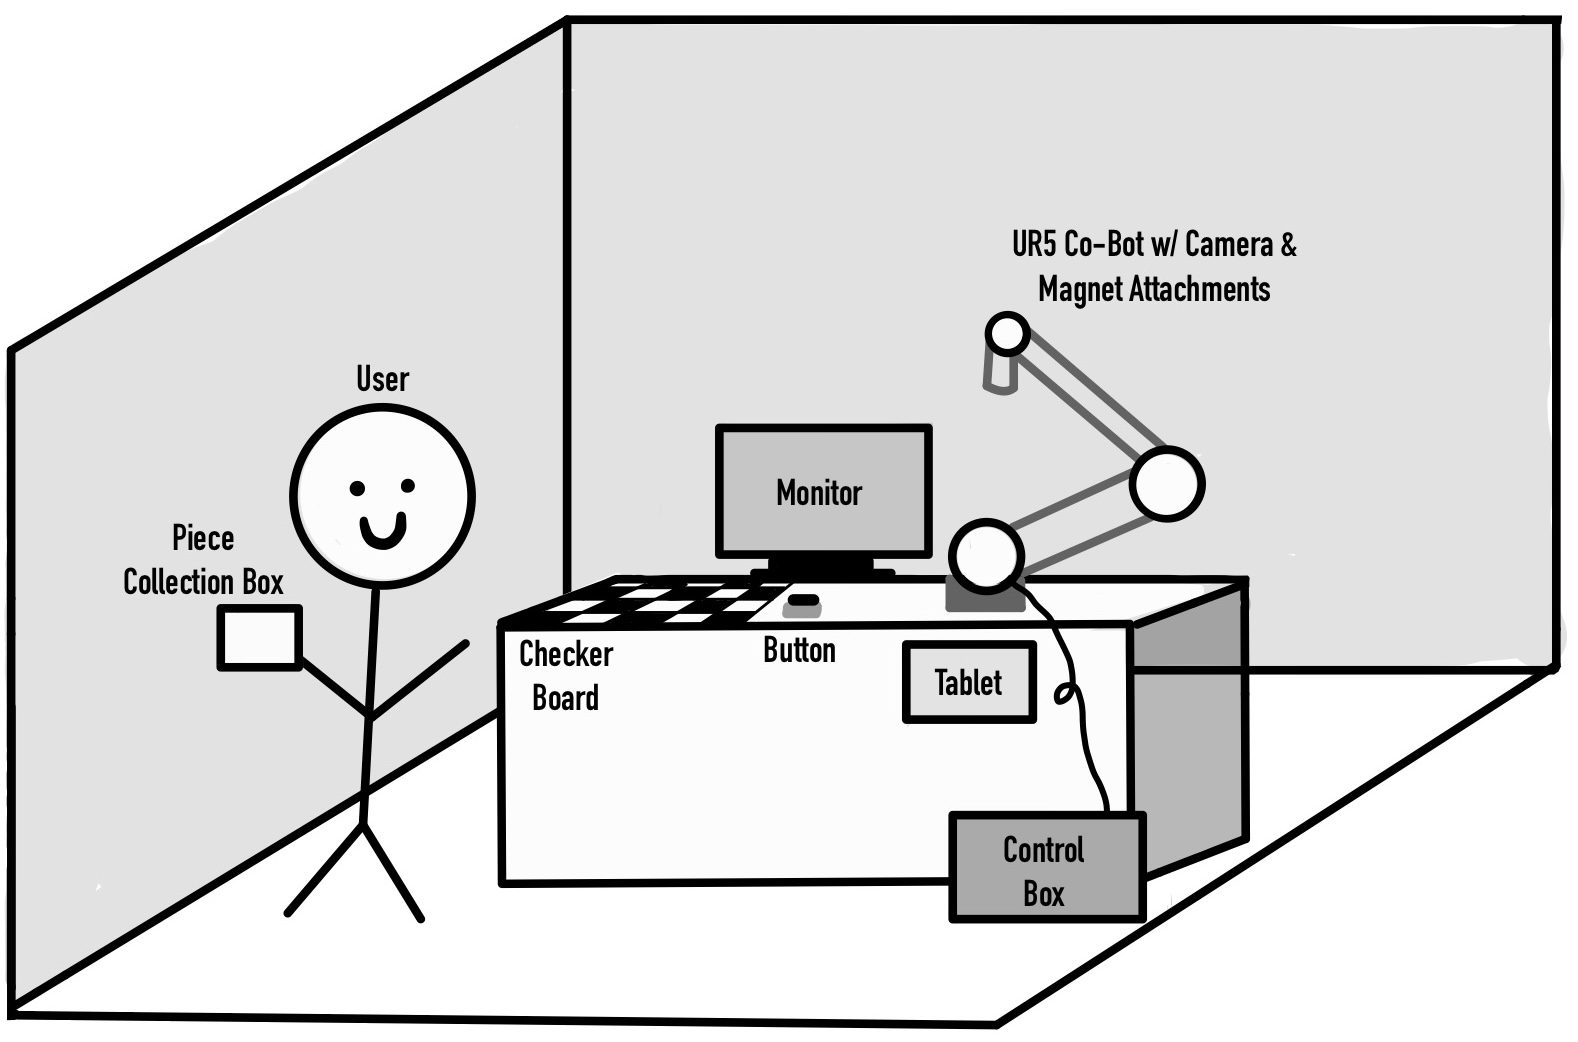
\includegraphics[width=0.70\textwidth]{images/Conceptual-Drawing.jpg}
    \caption{Conceptual Drawing}
\end{figure}

\section{System Overview}
% This section should reintroduce the full data flow diagram from the architectural specification, and discuss at a high level the purpose of each layer. You do not need to include a subsection for each layer, a 1 - 2 paragraph recap is sufficient.
\begin{flushleft}
The system for our product is currently simplified into 4 layers and 3 high-level components. Each layer/component will interact with one another in different ways.
\end{flushleft}
\begin{flushleft}
The Opponent is the person that will be going against the robot during the checkers game. The Input Device is one of the ways the opponent will be able to facilitate the progression of the checkers match. The camera is the component that acts as the eyes into the real world for our system. The Move Decision layer is the layer that will make all of the move decisions that the robot will make. This layer consists of Computer Vision and AI. The Computer layer is the central piece of our system. This layer acts as the facilitator of the checkers match, and receives input from the Opponent to progress the match, sends signals to the AI layer to grab board state and make a move, and signals the UR5 Robot Arm layer to execute those moves. The Move Execution layer is the layer that will physically execute the moves that our system will make during a checkers match with the robot arm and related parts. And finally, The External Components layer is composed of all of the physical checkers board game pieces. Both the Opponent component and the Move Execution layer physically interact with the External Components layer when they have made their move decisions to progress the match.
\end{flushleft}

\begin{figure}[h!]
	\centering
 	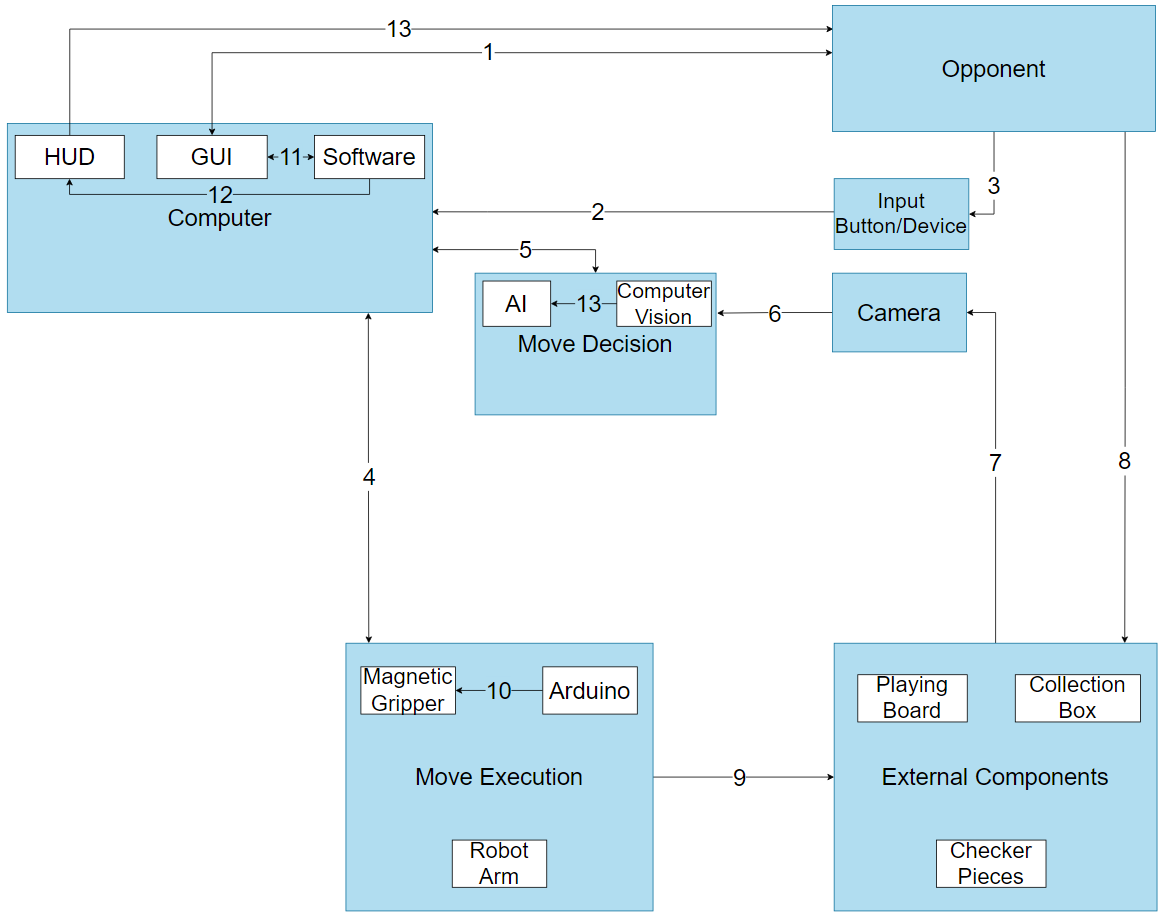
\includegraphics[width=0.90\textwidth]{images/data_flow_actual}
 \caption{System architecture}
\end{figure}

\newpage
%\section{Subsystem Definitions \& Data Flow}
%This section breaks down your layer abstraction to another level of detail. Here you grapically represent the logical subsytems that compose each layer and show the interactions/interfaces between those subsystems. A subsystem can be thought of as a programming unit that implements one of the major functions of the layer. It, therefore, has data elements that serve as source/sinks for other subsystems. The logical data elements that flow between subsystems need to be explicitly defined at this point, beginning with a data flow-like diagram based on the block diagram.

\begin{figure}[h!]
	\centering
 	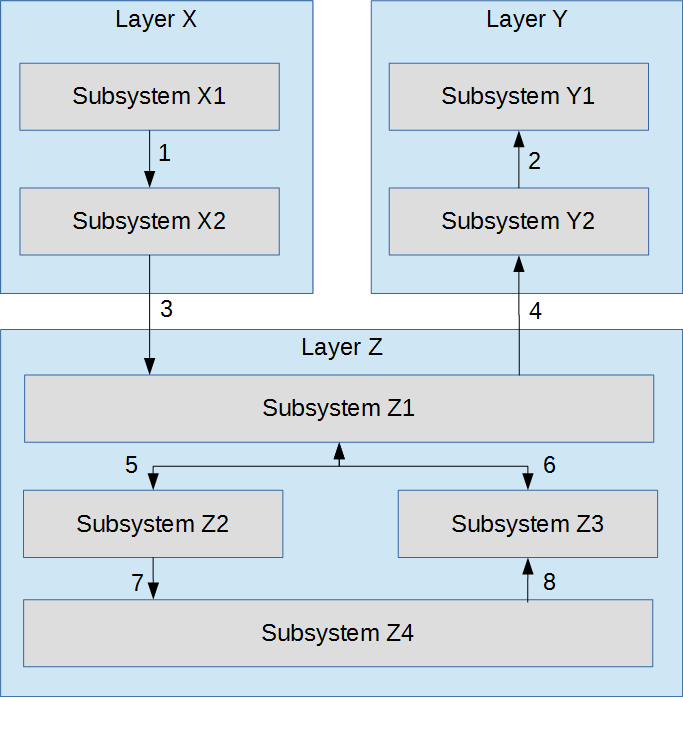
\includegraphics[width=\textwidth]{images/data_flow}
 \caption{A simple data flow diagram}
\end{figure}

\newpage
% \section{X Layer Subsystems}
%  In this section, the layer is described in terms of the hardware and software design. Specific implementation details, such as hardware components, programming languages, software dependencies, operating systems, etc. should be discussed. Any unnecessary items can be ommitted (for example, a pure software module without any specific hardware should not include a hardware subsection). The organization, titles, and content of the sections below can be modified as necessary for the project.

\subsection{Layer Hardware}
A description of any involved hardware components for the layer. For example, if each subsystem is a software process running on an embedded computer, discuss the specifics of that device here. Do not list a hardware component that only exists at the subsystem level (include it in the following sections).

\subsection{Layer Operating System}
A description of any operating systems required by the layer.

\subsection{Layer Software Dependencies}
A description of any software dependencies (libraries, frameworks, etc) required by the layer.

\subsection{Subsystem 1}
Descibe at a high level the purpose and basic design of this subsystem. Is it a piece of hardware, a class, a web service, or something else? Note that each of the subsystem items below are meant to be specific to that subystem and not a repeat of anything discussed above for the overall layer.

\begin{figure}[h!]
	\centering
 	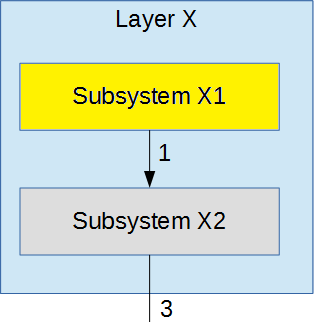
\includegraphics[width=0.60\textwidth]{images/subsystem}
 \caption{Example subsystem description diagram}
\end{figure}

\subsubsection{Subsystem Hardware}
A description of any involved hardware components for the subsystem.

\subsubsection{Subsystem Operating System}
A description of any operating systems required by the subsystem.

\subsubsection{Subsystem Software Dependencies}
A description of any software dependencies (libraries, frameworks, design software for mechanical parts or circuits, etc) required by the subsystem.

\subsubsection{Subsystem Programming Languages}
A description of any programming languages used by the subsystem.

\subsubsection{Subsystem Data Structures}
A description of any classes or other data structures that are worth discussing for the subsystem. For example, data being transmitted from a microcontroller to a PC via USB should be first be assembled into packets. What is the structure of the packets?

\subsubsection{Subsystem Data Processing}
A description of any algorithms or processing strategies that are worth discussing for the subsystem. If you are implementing a well-known algorithm, list it. If it is something unique to this project, discuss it in greater detail.



% \newpage
% \section{Y Layer Subsystems}
% In this section, the layer is described in terms of the hardware and software design. Specific implementation details, such as hardware components, programming languages, software dependencies, operating systems, etc. should be discussed. Any unnecessary items can be ommitted (for example, a pure software module without any specific hardware should not include a hardware subsection). The organization, titles, and content of the sections below can be modified as necessary for the project.

\subsection{Layer Hardware}
A description of any involved hardware components for the layer. For example, if each subsystem is a software process running on an embedded computer, discuss the specifics of that device here. Do not list a hardware component that only exists at the subsystem level (include it in the following sections).

\subsection{Layer Operating System}
A description of any operating systems required by the layer.

\subsection{Layer Software Dependencies}
A description of any software dependencies (libraries, frameworks, etc) required by the layer.

\subsection{Subsystem 1}
Descibe at a high level the purpose and basic design of this subsystem. Is it a piece of hardware, a class, a web service, or something else? Note that each of the subsystem items below are meant to be specific to that subystem and not a repeat of anything discussed above for the overall layer.

\begin{figure}[h!]
	\centering
 	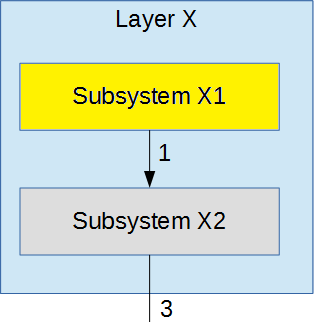
\includegraphics[width=0.60\textwidth]{images/subsystem}
 \caption{Example subsystem description diagram}
\end{figure}

\subsubsection{Subsystem Hardware}
A description of any involved hardware components for the subsystem.

\subsubsection{Subsystem Operating System}
A description of any operating systems required by the subsystem.

\subsubsection{Subsystem Software Dependencies}
A description of any software dependencies (libraries, frameworks, design software for mechanical parts or circuits, etc) required by the subsystem.

\subsubsection{Subsystem Programming Languages}
A description of any programming languages used by the subsystem.

\subsubsection{Subsystem Data Structures}
A description of any classes or other data structures that are worth discussing for the subsystem. For example, data being transmitted from a microcontroller to a PC via USB should be first be assembled into packets. What is the structure of the packets?

\subsubsection{Subsystem Data Processing}
A description of any algorithms or processing strategies that are worth discussing for the subsystem. If you are implementing a well-known algorithm, list it. If it is something unique to this project, discuss it in greater detail.



% \newpage
% \section{Z Layer Subsystems}
% In this section, the layer is described in terms of the hardware and software design. Specific implementation details, such as hardware components, programming languages, software dependencies, operating systems, etc. should be discussed. Any unnecessary items can be ommitted (for example, a pure software module without any specific hardware should not include a hardware subsection). The organization, titles, and content of the sections below can be modified as necessary for the project.

\subsection{Layer Hardware}
A description of any involved hardware components for the layer. For example, if each subsystem is a software process running on an embedded computer, discuss the specifics of that device here. Do not list a hardware component that only exists at the subsystem level (include it in the following sections).

\subsection{Layer Operating System}
A description of any operating systems required by the layer.

\subsection{Layer Software Dependencies}
A description of any software dependencies (libraries, frameworks, etc) required by the layer.

\subsection{Subsystem 1}
Descibe at a high level the purpose and basic design of this subsystem. Is it a piece of hardware, a class, a web service, or something else? Note that each of the subsystem items below are meant to be specific to that subystem and not a repeat of anything discussed above for the overall layer.

\begin{figure}[h!]
	\centering
 	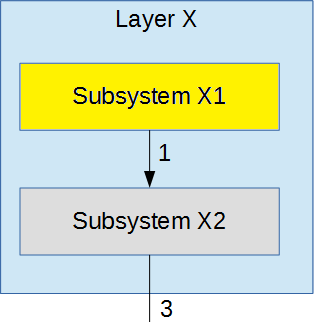
\includegraphics[width=0.60\textwidth]{images/subsystem}
 \caption{Example subsystem description diagram}
\end{figure}

\subsubsection{Subsystem Hardware}
A description of any involved hardware components for the subsystem.

\subsubsection{Subsystem Operating System}
A description of any operating systems required by the subsystem.

\subsubsection{Subsystem Software Dependencies}
A description of any software dependencies (libraries, frameworks, design software for mechanical parts or circuits, etc) required by the subsystem.

\subsubsection{Subsystem Programming Languages}
A description of any programming languages used by the subsystem.

\subsubsection{Subsystem Data Structures}
A description of any classes or other data structures that are worth discussing for the subsystem. For example, data being transmitted from a microcontroller to a PC via USB should be first be assembled into packets. What is the structure of the packets?

\subsubsection{Subsystem Data Processing}
A description of any algorithms or processing strategies that are worth discussing for the subsystem. If you are implementing a well-known algorithm, list it. If it is something unique to this project, discuss it in greater detail.



% \newpage
\section{Computer Layer Subsystems}
% In this section, the layer is described in some detail in terms of its specific subsystems. Describe each of the layers and its subsystems in a separate chapter/major subsection of this document. The content of each subsystem description should be similar. Include in this section any special considerations and/or trade-offs considered for the approach you have chosen.
In this section, the Computer layer is described in detail. This layer consists of the HUD, GUI, and Software subsystems. Overall, the layer is responsible for communicating with the players information about the state of the game, sending the robot arm the actions it needs to take, and handling the decisions after each move.


\subsection{HUD Subsystem}
% This section should be a general description of a particular subsystem for the given layer. For most subsystems, an extract of the architectural block diagram with data flows is useful. This should consist of the subsystem being described and those subsystems with which it communicates.

The Heads-Up Display (HUD) subsystem communicates with the Software subsystem of the Computer layer to receive information about the status of the game.

\begin{figure}[h!]
	\centering
 	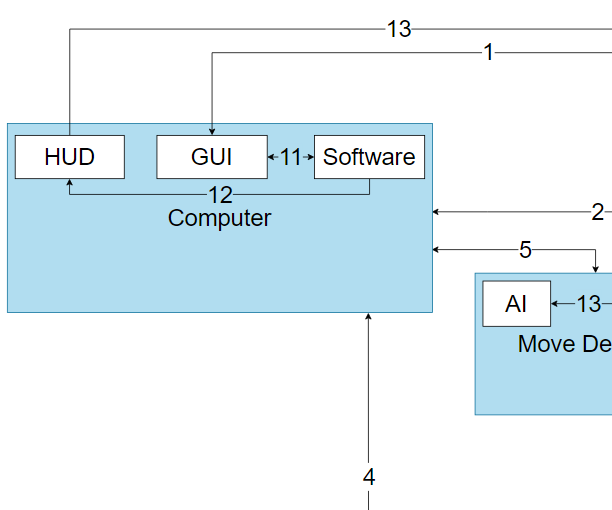
\includegraphics[width=0.80\textwidth]{images/computer_subsystems.png}
 \caption{Computer layer subsystems diagram}
\end{figure}

\subsubsection{Assumptions}
% Any assumptions made in the definition of the subsystem should be listed and described. Pay particular attention to assumptions concerning interfaces and interactions with other layers.

N/A
% The HUD information is able to be displayed on the computer screen to the user.

\subsubsection{Responsibilities}
% Each of the responsibilities/features/functions/services of the subsystem as identified in the architectural summary must be expanded to more detailed responsibilities. These responsibilities form the basis for the identification of the finer-grained responsibilities of the layer's internal subsystems. Clearly describe what each subsystem does.
The HUD subsystem displays to the user the status of the game and any information needed for the user. In this case the user is the Opponent layer. Information on the status of the game includes the current scores and a display of the game board on the computer monitor. This information is provided by the Software subsystem. When the physical game board changes, such as when a player moves a piece, this will also be reflected on the screen through the HUD.

\subsubsection{Subsystem Interfaces}
% Each of the inputs and outputs for the subsystem are defined here. Create a table with an entry for each labelled interface that connects to this subsystem. For each entry, describe any incoming and outgoing data elements will pass through this interface.

% \begin {table}[H]
% \caption {HUD Subsystem interfaces} 
% \begin{center}
%     \begin{tabular}{ | p{1cm} | p{6cm} | p{3cm} | p{3cm} |}
%     \hline
%     ID & Description & Inputs & Outputs \\ \hline
%     \#xx & Description of the interface/bus & \pbox{3cm}{input 1 \\ input 2} & \pbox{3cm}{output 1}  \\ \hline
%     \#xx & Description of the interface/bus & \pbox{3cm}{N/A} & \pbox{3cm}{output 1}  \\ \hline
%     \end{tabular}
% \end{center}
% \end{table}

Detailed in Table 2 are interfaces connected to the HUD subsystem. Incoming and outgoing data elements are detailed.

\begin {table}[H]
\caption {HUD Subsystem interfaces} 
\begin{center}
    \begin{tabular}{ | p{1cm} | p{6cm} | p{3cm} | p{3cm} |}
    \hline
    ID & Description & Inputs & Outputs \\ \hline
    \#12 & Information received from the Software subsystem to display & \pbox{3cm}{Game status and board} & \pbox{3cm}{N/A}  \\ \hline
    \#13 & Display game status through the Computer to the Opponent & \pbox{3cm}{N/A} & \pbox{3cm}{Game status and board}  \\ \hline
    \end{tabular}
\end{center}
\end{table}



\subsection{GUI Subsystem}
% Repeat for each subsystem
% This section should be a general description of a particular subsystem for the given layer. For most subsystems, an extract of the architectural block diagram with data flows is useful. This should consist of the subsystem being described and those subsystems with which it communicates.

The Graphical User Interface (GUI) subsystem is the main interactive component between the Computer and Opponent layers. It communicates with the Software subsystem within the Computer layer for its inputs and outputs.

\subsubsection{Assumptions}
% Any assumptions made in the definition of the subsystem should be listed and described. Pay particular attention to assumptions concerning interfaces and interactions with other layers.
The GUI only responds to keyboard inputs.

\subsubsection{Responsibilities}
% Each of the responsibilities/features/functions/services of the subsystem as identified in the architectural summary must be expanded to more detailed responsibilities. These responsibilities form the basis for the identification of the finer-grained responsibilities of the layer's internal subsystems. Clearly describe what each subsystem does.

The GUI is displayed on the monitor and can be interacted with by the use of keyboard keys by the player. These buttons will be able to change the state of the game for purposes such as new game, indicate their end of turn and quit game. Each time the opponent interacts with the GUI by sending a keyboard input for a specific function, this will interact with the computerized version of the game and update the game accordingly.

\subsubsection{Subsystem Interfaces}
% Each of the inputs and outputs for the subsystem are defined here. Create a table with an entry for each labelled interface that connects to this subsystem. For each entry, describe any incoming and outgoing data elements will pass through this interface.

Detailed in Table 3 are interfaces connected to the GUI subsystem. Incoming and outgoing data elements are detailed.

\begin {table}[H]
\caption {GUI Subsystem interfaces} 
\begin{center}
    \begin{tabular}{ | p{1cm} | p{6cm} | p{3cm} | p{3cm} |}
    \hline
    ID & Description & Inputs & Outputs \\ \hline
    \#1 & Opponent interacts with the GUI through keyboard inputs & \pbox{3cm}{Keyboard Input} & \pbox{3cm}{Game state change}  \\ \hline
    \#11 & Game state changes due to user interaction with the GUI & \pbox{3cm}{Keyboard Input} & \pbox{3cm}{Game state change}  \\ \hline
    \end{tabular}
\end{center}
\end{table}



\subsection{Software Subsystem}
% Repeat for each subsystem
% This section should be a general description of a particular subsystem for the given layer. For most subsystems, an extract of the architectural block diagram with data flows is useful. This should consist of the subsystem being described and those subsystems with which it communicates.

The Software subsystem is the main program behind the actions the UR5 Robot Arm will execute. This subsystem not only includes the source code itself, but also software packages needed for the program.

\subsubsection{Assumptions}
% Any assumptions made in the definition of the subsystem should be listed and described. Pay particular attention to assumptions concerning interfaces and interactions with other layers.
The subsystem is able to send instructions to the UR5 robot arm.

\subsubsection{Responsibilities}
% Each of the responsibilities/features/functions/services of the subsystem as identified in the architectural summary must be expanded to more detailed responsibilities. These responsibilities form the basis for the identification of the finer-grained responsibilities of the layer's internal subsystems. Clearly describe what each subsystem does.

The Software subsystem is responsible for handling events from the GUI. The subsystem also communicates with the UR5 robot arm through the Computer layer. The subsystem handles data on the status of the robot arm received from the robot arm itself. It also communicates to the robot arm what programmed actions it will need to perform. These actions will be determined by its interactions with the Move Decision layer which consists of the AI subsystem. The Software subsystem is also responsible for handling inputs from the Input Button/Device layer through the Computer layer.

\subsubsection{Software Subsystem Interfaces}
% Each of the inputs and outputs for the subsystem are defined here. Create a table with an entry for each labelled interface that connects to this subsystem. For each entry, describe any incoming and outgoing data elements will pass through this interface.

Detailed in Table 4 are related interfaces to the Software subsystem. Incoming and outgoing data elements are detailed.

\begin {table}[H]
\caption {Subsystem interfaces} 
\begin{center}
    \begin{tabular}{ | p{1cm} | p{6cm} | p{3cm} | p{3cm} |}
    \hline
    ID & Description & Inputs & Outputs \\ \hline
    \#2 & Signal that a turn has been completed by the Opponent & \pbox{3cm}{Keyboard Input pressed signal} & \pbox{3cm}{Signal to Move Decision layer}  \\ \hline
    \#4 & Communication between Move Execution and Computer layers & \pbox{3cm}{UR5 robot arm status} & \pbox{3cm}{Actions to be performed by the UR5 robot arm}  \\ \hline
    \#5 & Communication between Move Decision and Computer layers & \pbox{3cm}{Next move to make} & \pbox{3cm}{Game state change}  \\ \hline
    \#11 & Game state changes due to user interaction with the GUI & \pbox{3cm}{Keyboard Input signal} & \pbox{3cm}{Game state change}  \\ \hline
    \end{tabular}
\end{center}
\end{table}
\newpage
\section{Move Execution Layer Subsystems}
In this section, we describe the move execution layer. This layer is responsible for one of the key functionalities of our project which is the UR5 Robotic Arm's movement, which allows for the checkers game to take place between the user and the co-bot. The move execution layer is made up of three subsystems, the UR5 Robot Arm itself, the electromagnetic gripper, as well as an Arduino.

\subsection{Layer Hardware}
In terms of the Move Execution Layer the most heavily involved hardware component for this layer is the UR5 robotic arm itself. 

\subsection{Layer Operating System}
This layer utilizes Robot Operating System (ROS), although we do not primarily use ROS as we are primarily using Python to move our co-bot. ROS will be utilized to check the status of our robot's arm movements/coordinates at any given time.

\subsection{Layer Software Dependencies}
This layer will also utilize the Python 3.10.6 programming language. 

\begin{figure}[h!]
	\centering
 	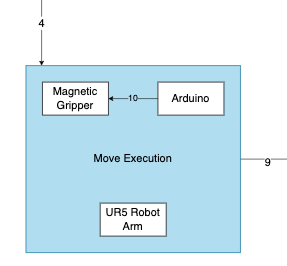
\includegraphics[width=0.60\textwidth]{images/move_execution.png}
 \caption{Move Execution subsystem description diagram}
\end{figure}

\subsection{UR5 Robot Arm}

The UR5 co-bot arm must be able to follow the instructions as asked by the software in order to hover over the correct location on the checker board. The robot must be able to move to fixed locations as predetermined by ROS and our custom software in order to not only move to specified pieces on the board but also to the collection box, and a waiting position.

The UR5 co-bot arm is responsible for the main mechanics of our project. As its ability to move to move to a spot on the board and pick up a piece and move it to another position is necessary so that the UR5 can play against its human oppponent.


\subsubsection{Subsystem Hardware}
In the UR5 Subsystem as well as the Move Execution Layer, the hardware component involved is the UR5 robotic arm itself.

\subsubsection{Subsystem Operating System}
The operating system required here is ROS.

\subsubsection{Subsystem Software Dependencies}
This subsystem layer will require a Universal Robots Python library so that we can control the co-bots movements through python scripts. The Python library we intend on using for this is ur\_rtde.

\subsubsection{Subsystem Programming Languages}
The UR5 subsystem requires the Python 3.10.6 programming language.

\subsubsection{Subsystem Data Structures}
The pre-recorded coordinates of our robot's movements will be saved into a multi-dimensional array so that our robot will have a list of saved positions to go to. The decision on where to go is determined by our Move Decision layer.

\subsubsection{Subsystem Data Processing}
N/A

\subsection{Magnetic Gripper}
The Magenetic subsystem of our Move Execution Layer is responsible for the UR5 robotic arm's ability to "pick-up" each checkers piece. This subsystem is integral to the project as a whole because without it the pieces will not be moved and the checkers game cannot be played.

\subsubsection{Subsystem Hardware}
This subsystem requires more hardware components than some of our other subsystems. It consists of an Arduino, an electromagnet, transistor NPN(2N3904), diode(1N4148), 22K Ω resistor, wires, breadboard, as well as a 3D printed attachement so that it can be screwed into the UR5 arm.

\subsubsection{Subsystem Operating System}
N/A

\subsubsection{Subsystem Software Dependencies}
This subsystem layer requires the Arduino 2.0.3 IDE. As that is needed for us to provide python scripts to Arduino which in turn will power our electromagnet.

\subsubsection{Subsystem Programming Languages}
The UR5 subsystem requires the Python 3.10.6 programming language.

N/A

\subsubsection{Subsystem Data Processing}
N/A
\newpage
\section{Move Decision Layer Subsystems}
 %In this section, the layer is described in terms of the hardware and software design. Specific implementation details, such as hardware components, programming languages, software dependencies, operating systems, etc. should be discussed. Any unnecessary items can be ommitted (for example, a pure software module without any specific hardware should not include a hardware subsection). The organization, titles, and content of the sections below can be modified as necessary for the project.
 In this section, we describe the move decision layer in detail. This layer consists of Artificial Intelligence and Computer Vision. Overall, this layer is responsible for one of the most important parts of this project that is the decision making process of the UR5 robot for the Checkers game. This does so by determining what commands to send to the robot arm.

\subsection{Layer Hardware}
%A description of any involved hardware components for the layer. For example, if each subsystem is a software process running on an embedded computer, discuss the specifics of that device here. Do not list a hardware component that only exists at the subsystem level (include it in the following sections).
This layer requires the computer to utilize artificial intelligence and computer vision aspects of the decision making.

\subsection{Layer Operating System}
%A description of any operating systems required by the layer.
The layer requires Linux distribution Ubuntu 22.04 LTS.

\subsection{Layer Software Dependencies}
%A description of any software dependencies (libraries, frameworks, etc) required by the layer.
The layer will use the Python 3.10.6 programming language. 

\subsection{Artificial Intelligence}
%Descibe at a high level the purpose and basic design of this subsystem. Is it a piece of hardware, a class, a web service, or something else? Note that each of the subsystem items below are meant to be specific to that subystem and not a repeat of anything discussed above for the overall layer.
The Artificial Intelligence communicates with the camera and Computer layer subsystems to make decisions for the UR5 robot arm.

\begin{figure}[h!]
	\centering
 	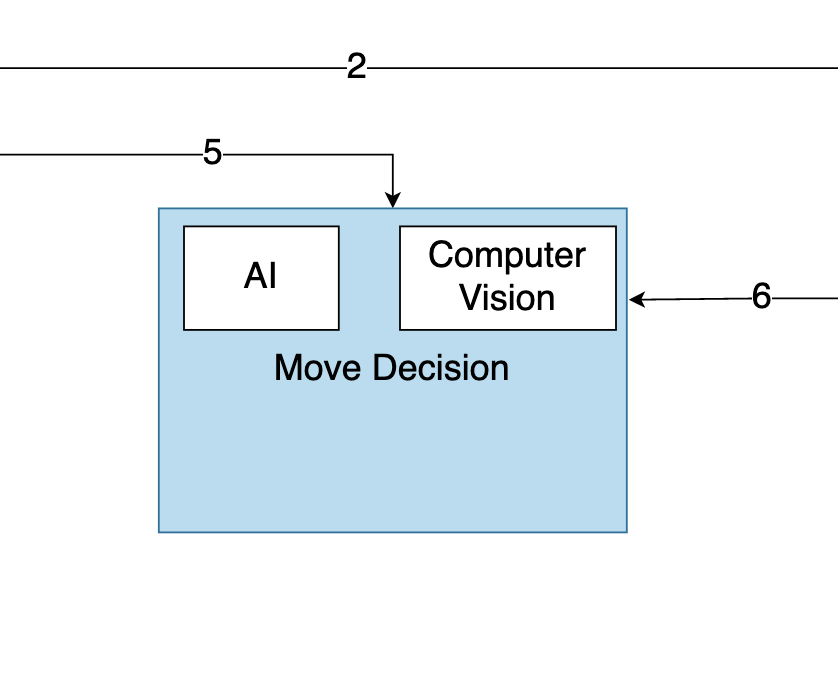
\includegraphics[width=0.60\textwidth]{images/move_decision.png}
 \caption{Example subsystem description diagram}
\end{figure}

\subsubsection{Subsystem Hardware}
%A description of any involved hardware components for the subsystem.
This subsystem requires the computer to utilize artificial intelligence aspect of the decision making.

\subsubsection{Subsystem Operating System}
%A description of any operating systems required by the subsystem.
The subsystem requires Linux distribution Ubuntu 22.04 LTS.

\subsubsection{Subsystem Software Dependencies}
%A description of any software dependencies (libraries, frameworks, design software for mechanical parts or circuits, etc) required by the subsystem.
The subsystem will use python libraries designed for artificial intelligence.

\subsubsection{Subsystem Programming Languages}
%A description of any programming languages used by the subsystem.
This subsystem will use the Python 3.10.6 programming language.

\subsubsection{Subsystem Data Structures}
%A description of any classes or other data structures that are worth discussing for the subsystem. For example, data being transmitted from a microcontroller to a PC via USB should be first be assembled into packets. What is the structure of the packets?
N/A

\subsubsection{Subsystem Data Processing}
%A description of any algorithms or processing strategies that are worth discussing for the subsystem. If you are implementing a well-known algorithm, list it. If it is something unique to this project, discuss it in greater detail.
N/A

\subsection{Computer Vision}
%Descibe at a high level the purpose and basic design of this subsystem. Is it a piece of hardware, a class, a web service, or something else? Note that each of the subsystem items below are meant to be specific to that subystem and not a repeat of anything discussed above for the overall layer.
The Computer Vision interacts with the frames received from the camera to determine the player's move.

% \begin{figure}[h!]
% 	\centering
%  	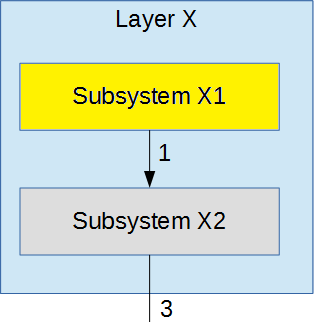
\includegraphics[width=0.60\textwidth]{images/subsystem}
%  \caption{Example subsystem description diagram}
% \end{figure}

\subsubsection{Subsystem Hardware}
%A description of any involved hardware components for the subsystem.
The subsystem will be using a camera to receive frames of the checkers position for both the players and will also use the computer for the computer vision process.

\subsubsection{Subsystem Operating System}
%A description of any operating systems required by the subsystem.
N/A

\subsubsection{Subsystem Software Dependencies}
%A description of any software dependencies (libraries, frameworks, design software for mechanical parts or circuits, etc) required by the subsystem.
This subsystem will use OpenCV and NumPy for the software dependencies.

\subsubsection{Subsystem Programming Languages}
%A description of any programming languages used by the subsystem.
This subsystem will use the Python 3.10.6 programming language.

\subsubsection{Subsystem Data Structures}
%A description of any classes or other data structures that are worth discussing for the subsystem. For example, data being transmitted from a microcontroller to a PC via USB should be first be assembled into packets. What is the structure of the packets?
N/A

\subsubsection{Subsystem Data Processing}
%A description of any algorithms or processing strategies that are worth discussing for the subsystem. If you are implementing a well-known algorithm, list it. If it is something unique to this project, discuss it in greater detail.
N/A




\newpage
\section{External Components Layer Subsystems}
In this section, the External Components layer is described in detail. This layer is comprised of the physical parts that make the checkers game, this includes the checkers playing board, the checkers pieces, and the collection box.

\subsection{Layer Hardware}
N/A or The components of this layer do now require any computer system hardware but it deals with the hardware of the checkers game, including the playing board, the checkers pieces, and the collection box.

\subsection{Layer Operating System}
N/A

\subsection{Layer Software Dependencies}
N/A

%%%%%%%%%%%%%%%%%%%%%%%%%%%%%%%%%%%%%%%%%
\subsection{Playing Board}
The Playing Board is the physical wooden platform with distinct cells which the checkers game is played upon. 

\begin{figure}[h!]
	\centering
 	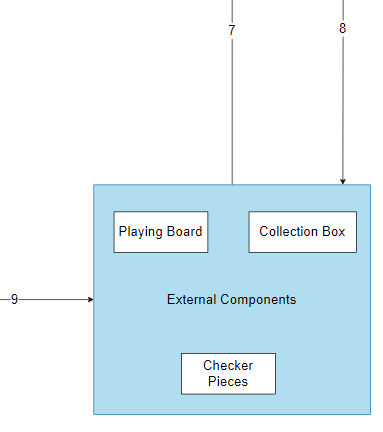
\includegraphics[width=0.60\textwidth]{images/externalComponents_subsystem.png}
 \caption{External components subsystem description diagram}
\end{figure}

\subsubsection{Subsystem Hardware}
% A description of any involved hardware components for the subsystem.
N/A

\subsubsection{Subsystem Operating System}
% A description of any operating systems required by the subsystem.
N/A

\subsubsection{Subsystem Software Dependencies}
% A description of any software dependencies (libraries, frameworks, design software for mechanical parts or circuits, etc) required by the subsystem.
N/A

\subsubsection{Subsystem Programming Languages}
% A description of any programming languages used by the subsystem.
N/A

\subsubsection{Subsystem Data Structures}
% A description of any classes or other data structures that are worth discussing for the subsystem. For example, data being transmitted from a microcontroller to a PC via USB should be first be assembled into packets. What is the structure of the packets?
N/A

\subsubsection{Subsystem Data Processing}
% A description of any algorithms or processing strategies that are worth discussing for the subsystem. If you are implementing a well-known algorithm, list it. If it is something unique to this project, discuss it in greater detail.
N/A

%%%%%%%%%%%%%%%%%%%%%%%%%%%%%%%%%%%%%%%%%
\subsection{Checkers Pieces}
The checkers pieces are the focus of the two players as they are the items that will be manipulated during the match. 

\subsubsection{Subsystem Hardware}
N/A

\subsubsection{Subsystem Operating System}
N/A

\subsubsection{Subsystem Software Dependencies}
% A description of any software dependencies (libraries, frameworks, design software for mechanical parts or circuits, etc) required by the subsystem.
N/A

\subsubsection{Subsystem Programming Languages}
% A description of any programming languages used by the subsystem.
N/A

\subsubsection{Subsystem Data Structures}
% A description of any classes or other data structures that are worth discussing for the subsystem. For example, data being transmitted from a microcontroller to a PC via USB should be first be assembled into packets. What is the structure of the packets?
N/A

\subsubsection{Subsystem Data Processing}
% A description of any algorithms or processing strategies that are worth discussing for the subsystem. If you are implementing a well-known algorithm, list it. If it is something unique to this project, discuss it in greater detail.
N/A

%%%%%%%%%%%%%%%%%%%%%%%%%%%%%%%%%%%%%%%%%
\subsection{Collection Box}
The collection box stands off to the side ready to hold the checkers pieces.

\subsubsection{Subsystem Hardware}
% A description of any involved hardware components for the subsystem.
N/A

\subsubsection{Subsystem Operating System}
% A description of any operating systems required by the subsystem.
N/A

\subsubsection{Subsystem Software Dependencies}
% A description of any software dependencies (libraries, frameworks, design software for mechanical parts or circuits, etc) required by the subsystem.
N/A

\subsubsection{Subsystem Programming Languages}
% A description of any programming languages used by the subsystem.
N/A

\subsubsection{Subsystem Data Structures}
% A description of any classes or other data structures that are worth discussing for the subsystem. For example, data being transmitted from a microcontroller to a PC via USB should be first be assembled into packets. What is the structure of the packets?
N/A

\subsubsection{Subsystem Data Processing}
% A description of any algorithms or processing strategies that are worth discussing for the subsystem. If you are implementing a well-known algorithm, list it. If it is something unique to this project, discuss it in greater detail.
N/A



\newpage
\section{Appendix A}
% Include any additional documents (CAD design, circuit schematics, etc) as an appendix as necessary.
\subsection{CAD Models}
\begin{figure}[h!]
	\centering
 	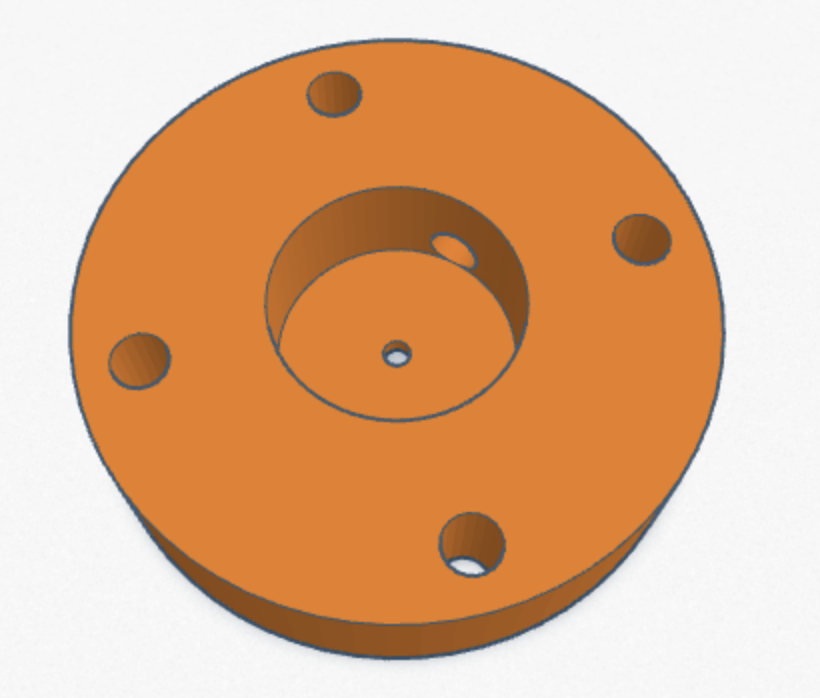
\includegraphics[width=0.30\textwidth]{images/Gripper Attachment.png}
 \caption{CAD Model of our Magnetic Gripper Attachment}
\end{figure}
\begin{figure}[h!]
	\centering
 	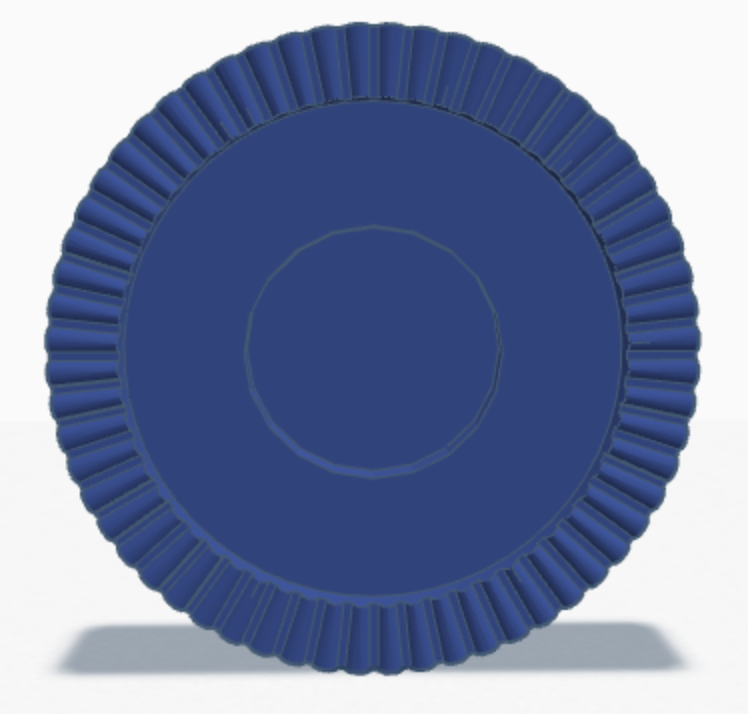
\includegraphics[width=0.30\textwidth]{images/Checkers Piece.png}
 \caption{CAD Model of our Regular Checkers Pieces}
\end{figure}
\begin{figure}[h!]
	\centering
 	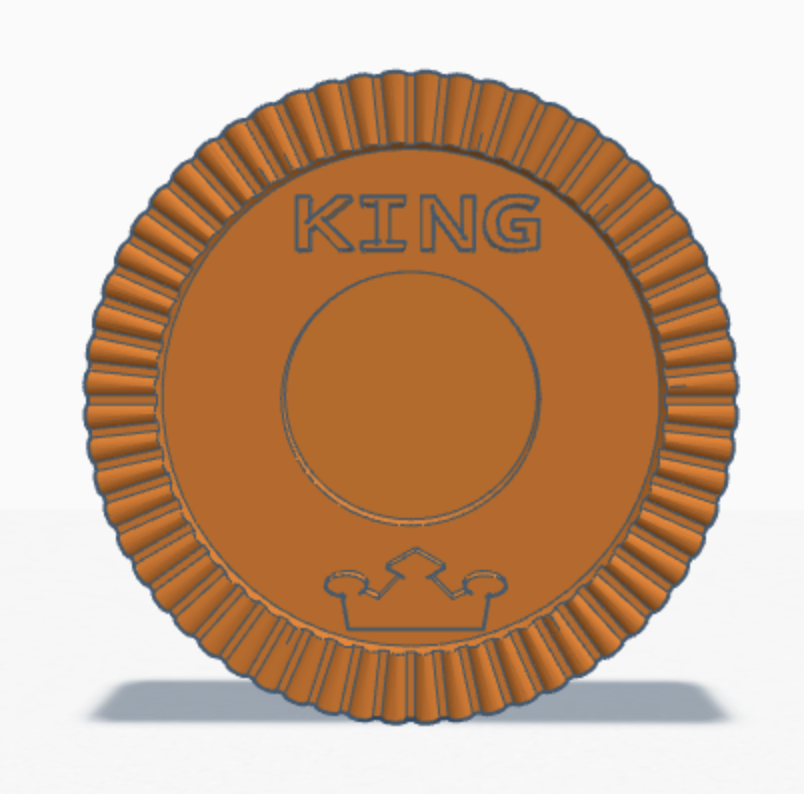
\includegraphics[width=0.30\textwidth]{images/King Piece.png}
 \caption{CAD Model of our King Checkers Pieces}
\end{figure}

\subsection{Circuit Schematics}
\begin{figure}[h!]
	\centering
 	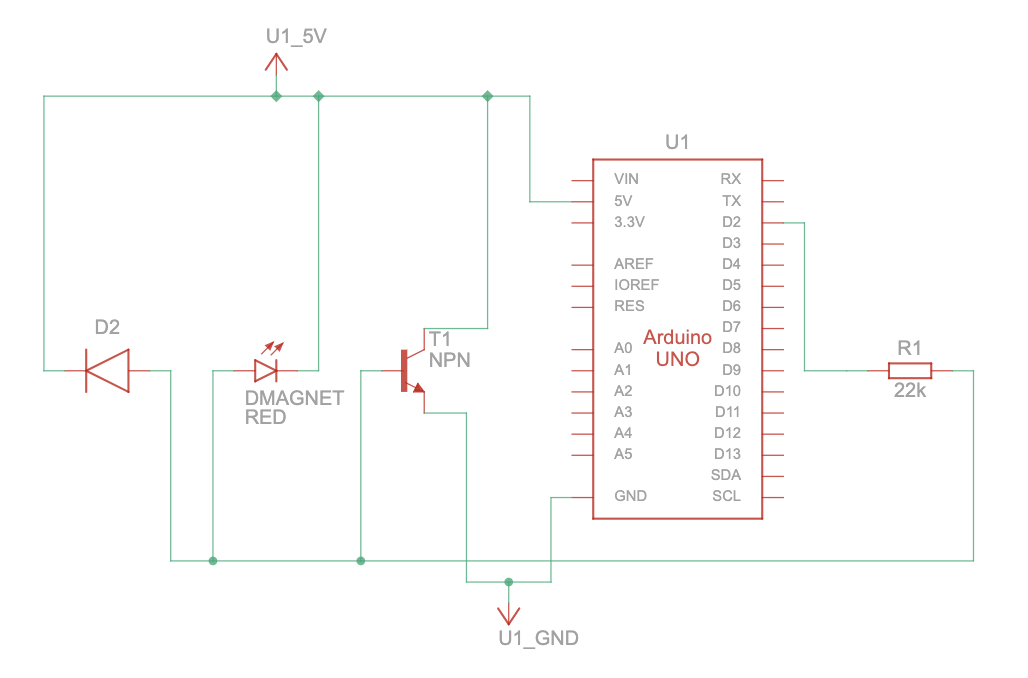
\includegraphics[width=1.00\textwidth]{images/Circut Schematic View.png}
 \caption{Schematic View of our Arduino \& Electromagnet setup}
\end{figure}
\begin{figure}[h!]
	\centering
 	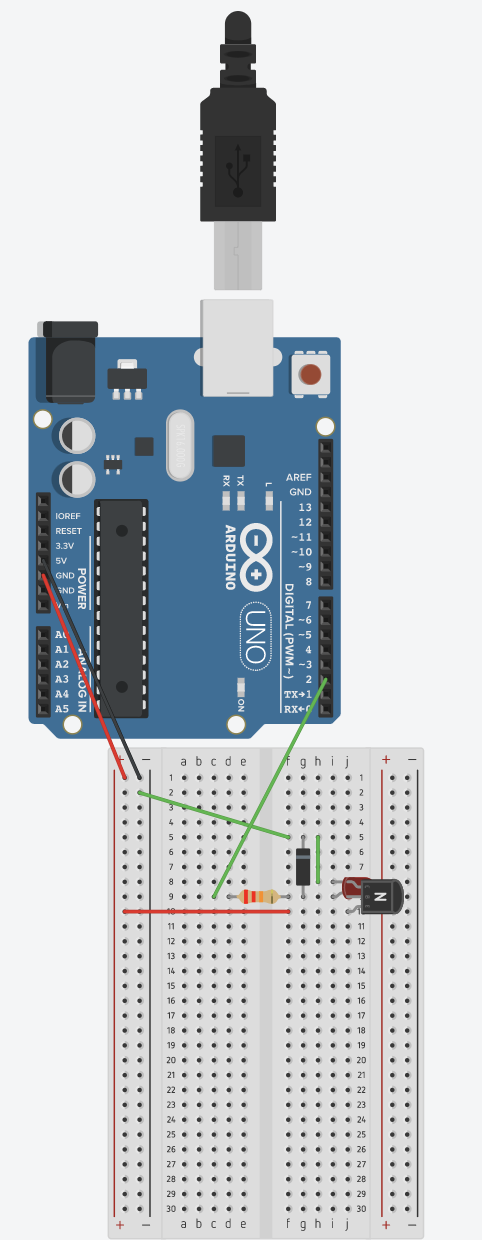
\includegraphics[width=0.40\textwidth]{images/Circut View.png}
 \caption{Circuit View of our Arduino \& Electromagnet setup}
\end{figure}
\newpage

%%% References
% \bibliographystyle{plain}
% \bibliographystyle{reference/IEEEtran_custom}
% \bibliography{reference/refs}{}

\end{document}